\section{Experiments and Discussion}

We evaluate eight agents in three environments. We record the regret accumulated by each agent as it runs and graph it. We present the regret vs. time graphs and show the relative ordering of each of the agents.

Among the eight agents the first two are trivial ones whose regret increases linearly with time. Every other agent is more intelligent and achieves sub-linear regret. We plot the regret vs. time graph of all agents except the first two since they are very trivial.

We run each agent for 20k rounds. Each environment takes about $\sim$10 minutes to run the simulation for all eight agents. We only focus on plotting the Unseen Regret of each arm, since we believe this is a stronger and more relevant notion of regret.

\subsection{The Agents}

The eight agents that we focus on are as follows.

\begin{enumerate}
    \item \textbf{Random Agent} picks an unseen arm half the times and a random seen arm otherwise.
    \item \textbf{Always New Arm Agent} always picks an unseen arm.
    \item \textbf{Naive UCB Agent} picks a new unseen arm with $p=1\%$ and every other time it picks among the known arms using UCB.
    \item \textbf{Naive Thompson Sampling Agent} picks a new unseen arm with $p=1\%$ and every other time it picks among the known arms using Thompson Sampling.
    \item \textbf{Fair UCB Agent} picks a new unseen arm with $p=1\%$ and every other time it picks among the known arms using UCB while also ensuring $\alpha$-Fairness among known arms.
    \item \textbf{Fair TS Agent} picks a new unseen arm with $p=1\%$ and every other time it picks among the known arms using Thompson Sampling while also ensuring $\alpha$-Fairness among known arms.
    \item \textbf{Surplus Curiosity UCB Agent} picks a new unseen arm with a probability based on the surplus, and every other time it picks among known arms using UCB.
    \item \textbf{Surplus Curiosity TS Agent} picks a new unseen arm with a probability based on the surplus, and every other time it picks among known arms using Thompson Sampling.
\end{enumerate}

\subsection{Environments}
The three environments that we evaluate the agents in are as follows.

\begin{enumerate}
    \item \textbf{Uniform Environment} is one in which every new arm has a quality $\mu$ which is sampled from a uniform distribution between $0$ and $1$.
    \item \textbf{Increasingly Better Environment} is one in which arms with bad quality are available in the begining and progressively better and better ones become available. In this environment every new arm has a quality $\mu$ which is sampled from a uniform distribution between $0$ and $T$, where $T$ starts from $0$ and increases slowly till $1$ by the time we reach the last round. 
    \item \textbf{Progressively Worse Environment} is the reverse of the previous environment. We start with good arms and later sampled arms go on getting worse and worse. Here $T$ starts from $1$ and decreases slowly till $0$ by the time we reach the last round. 
\end{enumerate}

\subsection{Results}

\subsubsection{Uniform Environment}
\begin{figure}[ht]
    \centering
    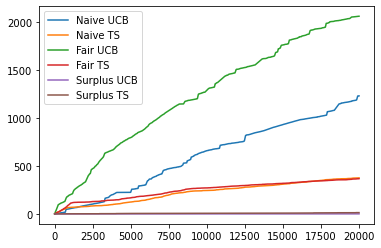
\includegraphics[width=0.8\columnwidth]{static-lin-lin.png}
    \caption{Uniform Environment. Linear-Linear Graph}
    \label{fig:u1}
\end{figure}

\begin{figure}[h!]
    \centering
    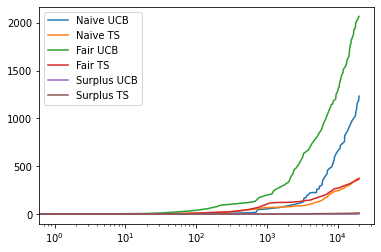
\includegraphics[width=0.8\columnwidth]{static-log-lin.png}
    \caption{Uniform Environment. Log-Linear Graph}
    \label{fig:u2}
\end{figure}

\begin{figure}[h!]
    \centering
    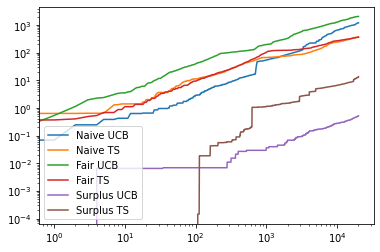
\includegraphics[width=0.8\columnwidth]{static-log-log.png}
    \caption{Uniform Environment. Log-Log Graph}
    \label{fig:u3}
\end{figure}

Figures 1 to 3 show the same data associated with the Uniform environment in three different scales. Only the relative ordering of each of the agents is important for us and not the precise numerical value of the regret associated with each arm. Thus we show the data in three different scales to highlight the ordering. The Y axis is the regret and the X axis is the number of rounds.

\subsubsection{Increasingly Better Environment}

\begin{figure}[ht]
    \centering
    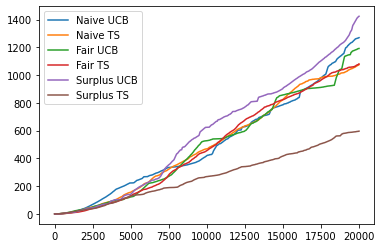
\includegraphics[width=0.8\columnwidth]{inc-lin-lin.png}
    \caption{Increasingly Better Environment. Linear-Linear Graph}
    \label{fig:i1}
\end{figure}

\begin{figure}[h!]
    \centering
    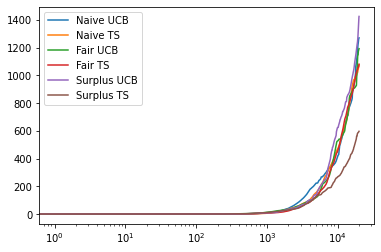
\includegraphics[width=0.8\columnwidth]{inc-log-lin.png}
    \caption{Increasingly Better Environment. Log-Linear Graph}
    \label{fig:i2}
\end{figure}

\begin{figure}[h!]
    \centering
    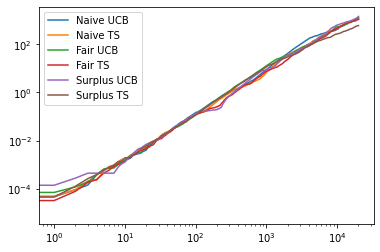
\includegraphics[width=0.8\columnwidth]{inc-log-log.png}
    \caption{Increasingly Better Environment. Log-Log Graph}
    \label{fig:i3}
\end{figure}

Similarly Figures 4 to 6 show regret vs. time graphs associated with the Increasingly Better Environment. 

\subsubsection{Progressively Worse Environment}

\begin{figure}[ht]
    \centering
    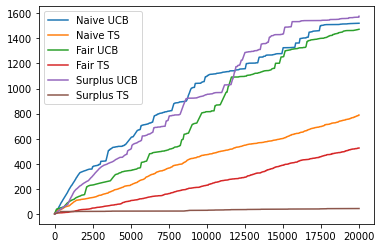
\includegraphics[width=0.8\columnwidth]{dec-lin-lin.png}
    \caption{Progressively Worse Environment. Linear-Linear Graph}
    \label{fig:d1}
\end{figure}

\begin{figure}[h!]
    \centering
    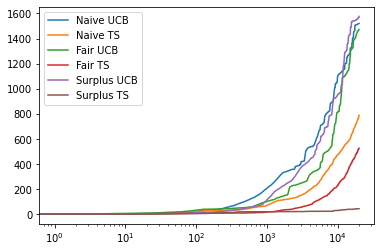
\includegraphics[width=0.8\columnwidth]{dec-log-lin.png}
    \caption{Progressively Worse Environment. Log-Linear Graph}
    \label{fig:d2}
\end{figure}

\begin{figure}[h!]
    \centering
    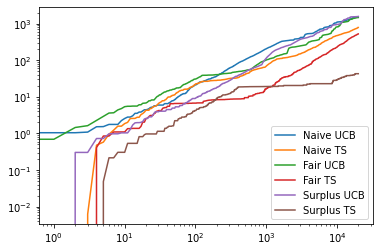
\includegraphics[width=0.8\columnwidth]{dec-log-log.png}
    \caption{Progressively Worse Environment. Log-Log Graph}
    \label{fig:d3}
\end{figure}

Figures 7 to 9 show the regret vs. time graphs in the Progressively Worse Environment.

\subsection{Discussion}
We observe the following trends from these graphs.

\begin{enumerate}
    \item Agents using Thompson Sampling perform better than those using UCB. \newcite{chat} make the claim that Thompson Sampling adapts better to the environment and performs better. We observe this in our experiments as well.
    \item There is a cost to ensuring fairness. Algorithms that incorporate fairness fare worse than their naive counterparts, although not by much. 
    \item Algorithms using the surplus weighted curiosity perform better than those that do not. Of these the Surplus Curiosity Thompson Sampling agent performs the best.
\end{enumerate}

